% !TeX spellcheck = en_US
\documentclass[11pt, a4paper]{article}
\usepackage[utf8]{inputenc}

\usepackage{latexsym}
\usepackage{float}
\usepackage[utf8]{inputenc}
\usepackage[english]{babel}
\usepackage{microtype}
\usepackage[hyphens]{url}
\usepackage{hyperref}
\usepackage{graphicx}
\usepackage[nonumberlist,acronym]{glossaries}
\usepackage{makeidx}
\usepackage{datetime}
\usepackage{multicol}
\usepackage{setspace}
\usepackage{pdflscape}
\usepackage{pgffor}
\usepackage{enumerate}
\usepackage{booktabs}
\usepackage{tabularx}
\usepackage{braket}
\usepackage{listings}
\usepackage{color}
\usepackage{amsmath}
\usepackage{amssymb}
\usepackage[table,xcdraw]{xcolor}
\usepackage{graphicx}
\usepackage{listings}
\usepackage{hyperref}
\usepackage{vmargin}
\usepackage{wrapfig}
\usepackage{subfiles}
\usepackage{float}
\usepackage{amsmath}
\usepackage{amssymb}
\usepackage{tikz-cd}
\usepackage{multirow}
\usepackage{pgffor}
\usepackage{enumitem}
\usepackage{iflang}
\usepackage{varioref}
\usepackage{hyperref}
\usepackage{cleveref}
\usepackage[justification=centering]{caption}
\usepackage{subcaption}
\usepackage{tikz}
\usepackage{enumitem}
\usepackage{xpatch}
\usepackage{refcount}
\usepackage{color}
\usepackage{pdfpages}
\usepackage{array}
\usepackage{eurosym}
\usetikzlibrary{mindmap}

%%%%%%%%%%%%%%%%%%%%%%%%%%%%%%%%%%%%%%%
%%%%%%%%%%%% UTIL COMMANDS %%%%%%%%%%%%  

\setcounter{secnumdepth}{4}
\newcommand{\nc}{\newcommand}
\nc{\supindex}{\textsuperscript}
\renewcommand{\baselinestretch}{1.5}
\nc{\myparagraph}[1]{\paragraph{#1}\mbox{}\\}

%%%%%%%%%%%%%%%%%%%%%%%%%%%%%%%%%%%%%%%
%%%%%%%%%%%%% CONFIG FILE %%%%%%%%%%%%%

\nc{\mytitle}{Economic Viability}
\nc{\mysubtitle}{Bayesian Inference}
\nc{\authors}{\textit{Oriol Alàs Cercós}}
\nc{\datetime}{25\supindex{th} of May, 2022}
\nc{\assignatura}{Technological Business Management and Entrepreneurship}
\nc{\professorat}{Josep Escribà Garriga}

% Per separar professors, utilitzar ','
% 	Ex: Maria, Joan, Pere

%%%%%%%%%%%%%%%%%%%%%%%%%%%%%%%%%%%%%%%
%%%%%%%%%%%%%  LANGUAGE   %%%%%%%%%%%%%

\newcommand{\tr}{\IfLanguageName{english}}

%%%%%%%%%%%%%%%%%%%%%%%%%%%%%%%%%%%%%%%
%%%%%%%%%%%%%%%%% MATH %%%%%%%%%%%%%%%%

\nc{\prob}[1]{P({#1})}
\nc{\probl}[2]{P({#1}|{#2})}

%%%%%%%%%%%%%%%%%%%%%%%%%%%%%%%%%%%%%%%
%%%%%%%%%%%%% FUNCTIONS %%%%%%%%%%%%

\nc{\numitems}[1]{\getrefnumber{#1}}
\newcounter{itemcntr}
\AtBeginEnvironment{itemize}{%
	\setcounter{itemcntr}{0}%
	\xapptocmd{\item}{\refstepcounter{itemcntr}}{}{}%
}

%%%%%%%%%%%%%%%%%%%%%%%%%%%%%%%%%%%%%%%
%%%%%%%%%%%%% RADIO BUTTON %%%%%%%%%%%%

\makeatletter
\newcommand*{\radiobutton}{%
	\@ifstar{\@radiobutton0}{\@radiobutton1}%
}
\newcommand*{\@radiobutton}[1]{%
	\begin{tikzpicture}
		\pgfmathsetlengthmacro\radius{height("X")/2}
		\draw[radius=\radius] circle;
		\ifcase#1 \fill[radius=.6*\radius] circle;\fi
	\end{tikzpicture}%
}
\makeatother


%%%%%%%%%%%%%%%%%%%%%%%%%%%%%%%%%%%%%%%
%%%%%%%%%%%%%  %%%%%%%%%%%%


\newcolumntype{S}{>{\centering\arraybackslash}m{1.5em}}

\renewcommand{\tabularxcolumn}[1]{m{#1}} % redefine 'X' to use 'm'
\newcommand{ \titem}[1]{\item \textbf{#1}\quad}


\newcolumntype{P}[1]{>{\centering\arraybackslash}p{#1}}

\setpapersize{A4}

\author{Oriol Alàs Cercós}
\date{29 d'Abril del 2019}

\makeglossaries
\newacronym{rs}{RS}{Remote Sensing}
\newacronym{sar}{SAR}{Synthetic Aperture Radar}
\newacronym{cnn}{CNN}{Convolutional Neural Network}
\newacronym{mlp}{MLP}{Multi-Layer Perceptron}
\newacronym{gan}{GAN}{Generative Adversarial Network}
\newacronym{cgan}{cGAN}{Conditional Generative Adversarial Network}
\newacronym{mcgan}{McGAN}{Multi-spectral Conditional Generative Adversarial Network}
\newacronym{nir}{NIR}{Near Infra Red}
\newacronym{ir}{IR}{Infra Red}
\newacronym{l1c}{L1C}{Level-1C}
\newacronym{l2a}{L2A}{Level-2A}
\newacronym{nlp}{NLP}{Natural Language Processing}
\newacronym{psnr}{PSNR}{Peak signal-to-noise ratio}
\newacronym{ssim}{SSIM}{Structural Similarity Index Metric}
\newacronym{rnn}{RNN}{Recurrent Neural Network}
\newacronym{vit}{ViT}{Vision Transformer}
\newacronym{ltae}{L-TAE}{Lightweight Temporal Attention Encoder}
\newacronym{tae}{TAE}{Temporal Attention Encoder}
\newacronym{vae}{VAE}{Variational AutoEncoder}


\def\contentsname{Índex}
\begin{document}
	
	\definecolor{gray}{rgb}{0.4,0.4,0.4}
	\definecolor{darkblue}{rgb}{0.0,0.0,0.6}
	\definecolor{cyan}{rgb}{0.0,0.6,0.6}
	\lstset{
		basicstyle=\ttfamily,
		columns=fullflexible,
		showstringspaces=false,
		commentstyle=\color{gray}\upshape
	}
	
	\lstdefinelanguage{XML}
	{
		morestring=[b]",
		morestring=[s]{>}{<},
		morecomment=[s]{<?}{?>},
		stringstyle=\color{black},
		identifierstyle=\color{darkblue},
		keywordstyle=\color{cyan},
		morekeywords={xmlns,version,type}% list your attributes here
	}
	
	\begin{titlepage}
		\begin{figure}[htb]
			\begin{center}
				
				\includegraphics[width=5cm]{imgs/udl.png}\\
				
				
				\medskip
				\begin{center}
					
					\huge\textbf{\mytitle}\\
					\bigskip
					\normalsize{\tr{Made by}{Realitzat per:}}
					\\
					\large\textit{\authors}
					\\
					\setlength{\parskip}{1em}
					\normalsize{\tr{Delivery}{Data de lliurament:}}
					\\
					\large{\datetime}
				\end{center}
				
				\vspace*{\stretch{2.0}}
			\end{center}
		\end{figure}
		\begin{flushright}
			Universitat de Lleida
			\\
			Escola Politècnica Superior
			\\
			Màster en Enginyeria Informàtica
			\\
			\assignatura
			\\
			\medskip
			\textbf{\tr{Professorate:}{Tutor:}}
			\\
			\foreach \n in \professorat{\n\\}
		\end{flushright}
		\thispagestyle{empty} 
	\end{titlepage}
	\pagenumbering{roman}
	\tableofcontents
	\listoffigures
	\listoftables
	\newpage
	\printglossary[type=\acronymtype]
	\newpage
	\pagenumbering{arabic}
	\section{Introduction} 
	\gls{rs} imagery is critical to perform challenges such climate change or natural resources management, including zone monitoring for reforestation, disaster mapping, land surface change detection and coastal water quality monitoring.  % canvi de terrenys, natural resources management, climate change, zone monitoring for reforestation, climate change, disaster mitigation 
	Nevertheless, on average 55\% of the Earth's land surfaces is covered by clouds, being then a significant impediment to carry out a broad range of applications. Satellite imagery plagued by films of clouds that obstructs the scene implies a great loss of information or causing effects such as blurring, which mitigates the power of \gls{rs}. Hence, \gls{rs} applications definitely needs a generic technique to detect and remove the cloudy region with an in-painting of the underlying scene.
	\\
	\\
	Once set the problem, the goals of this master thesis have been:
	\begin{itemize}
		\item Search state-of-the-art solutions as well as frameworks that could bring new improvements and better results.
		\item Create or search for a multi-temporal and spatial imagery to design and evaluate a model that can remove the clouds given a satellite image.
		\item Design and implement an effective model and monitoring its training.
		\item Evaluate the model and make a comparison with the other solutions proposed.
	\end{itemize}

	\newpage
	\section{Problem Analysis}
	\subsection{Sentinel2}
	The analysis of the problem has been focused using Copernicus Sentinel2 constellation. 
	Sentinel2 images are provided by two satellites, Sentinel 2A and Sentinel 2B, which orbit each other with a 180º phase shift. Generally, the acquisition of the images is more or less 10 days per satellite so that a new updated image of a specific area is available in periods of time not exceeding five days. This makes Sentinel-2 data an excellent choice for studying environmental challenges. Sentinel-2 products are a compilation of elementary granules of fixed size, within a single orbit. A granule, also called tile, is a multi-spectral image with 13 bands in the visible, near-infrared, and short-wave infrared spectrum. These bands come in a different spatial resolution ranging from 10m to 60m, so the images can be classified as medium-high resolution. All the granules are 100x100km2 ortho-images in UTM/WGS84 projection. There are five types of Sentinel-2 data although only two are available for users: \gls{l1c} and \gls{l2a}. The difference between them is that the latter provides background reflectance imagery of the atmosphere derived from associated \gls{l1c} products. In \ref{tab:sentinel2-bands}, there are the bands with its most high resolution and ordered by its central wavelength, being B5-B12 \gls{nir} or \gls{ir} bands.
	\begin{table}[H]
		\centering
		\caption{Sentinel 2 bands}
		\label{tab:sentinel2-bands}
		\begin{tabular}{llrrr}
			\hline
			Band & Name                & \parbox{3cm}{\centering \vspace{0.5cm} Central \\ wavelength ($\mu m$) \\ \hspace{0.1cm}} & Bandwidth (nm) & \parbox{3cm}{\centering Spatial\\ resolution (m)} \\ \hline
			B1   & Coastal aerosol     &                      $0.433$ &             27 &                     60 \\
			B2   & Blue                &                        0.490 &             98 &                     10 \\
			B3   & Green               &                        0.560 &             45 &                     10 \\
			B4   & Red                 &                        0.665 &             38 &                     10 \\
			B5   & Vegetation Red Edge &                        0.705 &             19 &                     20 \\
			B6   & Vegetation Red Edge &                        0.740 &             18 &                     20 \\
			B7   & Vegetation Red Edge &                        0.783 &             28 &                     20 \\
			B8   & NIR                 &                        0.842 &            125 &                     10 \\
			B8A  & Vegetation Red Edge &                        0.865 &             33 &                     20 \\
			B9   & Water Vapour        &                        0.945 &             26 &                     60 \\
			B10  & SWIR-Cirrus         &                        1.375 &             75 &                     60 \\
			B11  & SWIR                &                        1.610 &            143 &                     20 \\
			B12  & SWIR                &                        2.190 &            242 &                     20\\\hline
		\end{tabular}
	\end{table}
The bands can give us a various range of aspects of the orthogonal view. Several spectral indices have been created over the years by performing operations between the bands, which can broaden the range of analysis and make them more accurate to finally better understand the features in the imagery. The most used bands to generate indices are B3, B4 and B8. The following list explains some of the most popular:
\begin{description}
		\item[NDVI] The Normalized Difference Vegetation Index is highly associated with the vegetation content. Higher values of NDVI correspond to areas that reflect more in the near-infrared spectrum and to denser and healthier vegetation.
		\[\text{NDVI} =  \frac{\text{B8} - \text{B4}}{\text{B8} + \text{B4}}\] 
		\item[GNDVI] Green Normalized Difference Vegetation Index is modified version NDVI to be more sensitive to the variation of chlorophyll content in the crop.
		\[\text{GNDVI} =  \frac{\text{B8} - \text{B3}}{\text{B8} + \text{B3}}\] 
		\item[NDMI] Normalized Difference Moisture Index is used to determine vegetation water content.
		\[\text{NDMI} = \frac{\text{B8} - \text{B11}}{\text{B8} + \text{B11}}\]
		\item[MSI] Moisture Stress Index increases in leaf water content, so that makes it perfect for finding water stress in plants.
		\[\text{MSI} = \frac{\text{B11}}{\text{B8}}\]
		\item[NBRI] Normalized Burned Ratio Index detects burned areas and it is used to monitor the recovery of the ecosystem.
		\[\text{NBRI} = \frac{\text{B8} - \text{B12}}{\text{B8} - \text{B12}}\]
		\item[BSI] Bare Soil Index quantifies the soil mineral composition and the presence of vegetation.
		\[\text{BSI} = \frac{(\text{B11} + \text{B4} )- (\text{B8} + \text{B2})}{(\text{B11} + \text{B4} ) + (\text{B8} + \text{B2})}\]
		\item[NDWI] Normalized Difference Water Index is used for the identification of water bodies although is sensitive to build-up land and result in over-estimated water bodies.
		\[\text{NDWI} = \frac{\text{B3} - \text{B8}}{\text{B3} + \text{B8}}\]
		\item[NDSI] Normalized Difference Snow Index identifies snow cover over land areas since in B11 snow absorbs most of the incident radiation while the clouds do not.
		\[\text{NDSI} = \frac{\text{B3} - \text{B11}}{\text{B3} + \text{B11}}\]
\end{description}
	\subsection{Related work and state-of-the-art}
	\subsubsection{Deep Learning \& CNN}
	Deep learning have been a popular and efficient technique to solve challenges from satellite imagery. Specifically, \gls{cnn} have been the main architecture of neural networks to provide a solution from image-based problems. What differentiates \gls{cnn} from the standard \gls{mlp} is that they have hidden layers called convolutional layers, which are able to take patterns from their inputs using filters. A filter can be considered a relatively small matrix that slides from the input by operating with the weights of the matrix. This action is called \textit{convolving }and, in its simplest case, the output value of a layer with ($N, C_{in}, H, W$) as the input and ($N, C_{out}, H_{out}, W_{out}$) as the output is described as:
	\[out(N_i, C_{out_j}) = bias(C_{out_j}) + \sum_{k=0}^{C_{in} - 1} weight(C_{out_j}, k) \star \, input(N_i, k)\]
	where $\star$ is the 2D cross-correlation operator, $N$ is the batch size, $C$ denotes the number of channels and $H$ and $W$ are the height and width in pixels of the planes respectively. A graphic representation of a CNN architecture can be seen in \ref{fig:related-lenet}
	\begin{figure}[H]
		\centering
		\includegraphics[width=14cm]{imgs/relatedwork/lenet-5.jpeg}
		\caption{LeNet-5 architecture.}
		\label{fig:related-lenet}
	\end{figure}
	Being that told so, there are a lot of state-of-the-art using \gls{cnn}. In \cite{LANARAS2018305}, they create a deep learning approach to Sentinel-2 super-resolution. Their hypothesis was the existence of a complex mixture of correlations across many spectral bands over a large spatial context. Hence, the input of the model is a concatenation of the high-level resolution bands with the low-level resolution bandwidths upsampled to 10m by simple bi-linear interpolations. The model itself is a clear reference of residual networks \cite{he2016deep}.
	\begin{figure}[H]
		\centering
		\includegraphics[width=6cm]{imgs/relatedwork/residualblock.png}
		\caption{Residual learning: a building block.}
	\end{figure}
	Residual architectures use contiguous blocks of the convolution layers with the same properties. This layers are connected also with skip connections to reduce the average effective path length through the network, alleviate the vanishing gradient problem and greatly accelerates the learning during the training.  As it can be seen in \ref{fig:related-residual-loss}, networks without skip connections are harder to train as the loss surface is to hard to navigate. \cite{NEURIPS2018_a41b3bb3}
	\begin{figure}[H]
		\centering
		\includegraphics[width=10cm]{imgs/relatedwork/resloss.png}
		\caption{Loss surfaces of ResNet-56 with/without skip connections.}
		\label{fig:related-residual-loss}
	\end{figure}
	Similarly, in \cite{Meraner2020}, a residual network is used with the same skip connections mechanism to bring a solution to cloud removal challenge.
	Regarding the design of the neural network, DSen2-CR is a fully convolutional network, so it can accept input images of any spatial dimensions (\textit{m}), as it can be seen in \ref{fig:related-dsen2-cr}.
	The  output of DSen2-CR is a 13-channel layer, representing the thirteen bands from Sentinel2.  
	\begin{figure}[H]
		\centering
		\includegraphics[width=10cm]{imgs/relatedwork/sar.png}
		\caption{DSen2-CR model diagram.}
		\label{fig:related-dsen2-cr}
	\end{figure}
	 It also uses
	\gls{sar} 
	optical data, which represents an important complementary source to help the model to make greater results. However, \gls{sar} images are affected by a particular type of noise called \textit{speckle}, which can difficult network's learning and effectiveness. In addition to that, the model depends on one more source to remove the clouds, as \gls{sar} images cannot be downloaded in Sentinel-2. It can be seen in \ref{fig:related-dsen2-cr-predictions} that the lack of \gls{sar} data make the network less powerful. 
	\begin{figure}[H]
		\centering
		\includegraphics[width=13cm]{imgs/relatedwork/dsen2-cr-predictions.png}
		\caption{Examples of the influence of SAR data. Being (a, f) cloudy images, (b, g), SAR images, (c, h), the target cloudless images, (d, i), the synthesized images without SAR input data and (e, j) the predictions using SAR data as input.}
		\label{fig:related-dsen2-cr-predictions}
	\end{figure}
	\subsubsection{Generative Adversarial Networks}
	Improvements have been found using \gls{gan} \cite{goodfellow2014generative}, which is a model architecture that belongs to the set of generative models. Generative models are a class of machine learning that learn a representation of the data trained on and they model the data itself. \gls{gan} is an unsupervised model made up of two neural networks: the generator and the discriminator. The idea is based on a game theoretic scenario in which the generator network must compete against an adversary. While the generator network produces samples, the aim of the discriminator is to distinguish between the real samples and the drawn by the generator. The discriminator is a binary classifier trying not to be fooled. 
	\begin{figure}[H]
		\centering
		\includegraphics[width=11cm]{imgs/relatedwork/gan.png}
		\caption{GAN model diagram.}
		\label{fig:related-gan-diagram}
	\end{figure}
	The generator loss is calculated using the discriminator as a reference of how much far is from real images while the discriminator loss is calculated by how much accurate is discerning between the synthesized data and the real one. The standard function can be known as the min-max loss:
	\begin{align*}
		Loss_D(D) =& \; E_x[log(D(x)]\\
		Loss_G(G) =& \; E_y[log(1 - D(G(y)))]\\
		Loss_{GAN}(G, D) =&\; Loss_D(D) + Loss_G(G)
	\end{align*}
	During training, both networks constantly try to outsmart each
	other, in a zero-sum game. At some point of the training, the game may end up in a state that
	game theorists call a Nash equilibrium, when no player would be better off changing their own strategy, assuming the other players do not change theirs. \gls{gan}s can only reach one possible Nash equilibrium: when the generator produces so realistic images that the discriminator is forced to guess by 50 \% probability that the image is real or not. Nevertheless, the training process not always can converge to that equilibrium. There are several factors that make the training hard to reach the desired state. For instance, there is a possibility that the discriminator always outsmarts the generator so that it can clearly distinguish between fake and real images. As it never fails, the generator is stuck trying to produce better images as it cannot learn from the errors of the discriminator. Possible solutions can be carried out such as making the discriminator less powerful, decreasing the learning rate or adding noise to the discriminator target. Another big obstacle is when the generator becomes less diverse, and it learns only to perfectly generate realistic images of a single class, so it forgets about the others. This is  called \textit{mode collapse}. At some point, the discriminator can learn how to beat the generator, but then, the latter is forced to do the same but in another class, cycling between classes never becoming good at any of them. A popular technique to avoid is \textit{experience replay}, which consists in storing synthetic images at each iteration in a replay buffer. There is a lot of literature of obstacles and solutions to improve \gls{gan} training and it is still very active, as it is in its applications too. The tuning of hyper-parameters and the design of the model will be a key to pursue the Nash equilibrium. For instance, there is a variant called \gls{cgan}. Traditionally, the generative network only produces the image from a random vector as an input, which is also called \textit{latent vector} since it cannot be manipulated or with prior convictions of how will be. Unfortunately, this only allows to generate a random image from the domain of the latent space, which is hard to map to the generated images. However, \gls{cgan} can be trained so that both generator and discriminator models can be conditioned to some class labels or multi-dimensional vectors and produce synthetic images from a specific domain. In \ref{fig:related-cgan-diagram}, it can be seen a \gls{cgan} diagram where the generator is conditioned by some inputs as well as the real data have the condition vector in each sample.
	\begin{figure}[H]
		\centering
		\includegraphics[width=11cm]{imgs/relatedwork/cgan.png}
		\caption{cGAN model diagram.}
		\label{fig:related-cgan-diagram}
	\end{figure}	
	Actually, it is hard to find another \gls{gan} that can fit better in cloud removal problem without being \gls{cgan}, since the model needs to be conditioned to the input image. In \cite{8014931}, they %TODO change name
	proposed a  \gls{mcgan} trained using RGB and \gls{nir} cloud-free bands as input and synthetic RBG cloudy images as target. It is true that short wave bands are unaffected by cloud cover and using \gls{nir} images to guide to uncover the clouds of satellite imagery is great since \gls{nir} bands posses have higher penetration through fog than visible light bands. Nevertheless, synthesizing the target might not be realistic enough to feasibly deploy the model in real-state. Regarding the experimental results, they have only showed qualitative metrics by comparing the ground-truth with cloud-free images, ones synthesized and ones real, accompanied both by the cloud obscure image and the cloud mask.  As the NIR channel is not altered by the perlin noise, there is a huge difference about the effectiveness comparing the synthesized images with the real ones, as it can be seen in \ref{fig:related-mcgan-synthesized} and \ref{fig:related-mcgan-real}
	\begin{figure}[H]
		\centering
		\includegraphics[width=12cm]{imgs/relatedwork/mcgan-synthesized.png}
		\caption{Prediction results by McGAN with the synthesized cloud images}
		\label{fig:related-mcgan-synthesized}
	\end{figure}
	\begin{figure}[H]
	\centering
	\includegraphics[width=12cm]{imgs/relatedwork/mcgan-real.png}
	\caption{Prediction results by McGAN with the real cloud images}
	\label{fig:related-mcgan-real}
\end{figure}
	To overcome the need of synthesized data, \cite{sarukkai2019cloud} proposed two datasets and two models respective to each of the datasets. Both neural networks have versions depending on including or excluding the \gls{nir} channel as an input. The first is based on Pix2Pix \cite{pix2pix2017} model, a \gls{cgan} which performs very well in image-to-image translation tasks. The generator network of Pix2Pix  uses a encoder-decoder architecture but with skip-connections to avoid loss of information of the bottleneck, similar to U-Net architecture \cite{unet}. The model is trained by a paired dataset of single-images. That means the dataset have a cloudy image as input and a real cloud-free image of the same zone. The generator tries to produce the image as real as the target ones, so it is compulsory to have both images.  The second model proposed is a spatio-temporal \gls{cgan} trained by pairing clear images with three cloudy corresponding from diverse points in time. Instead of only trying the U-Net architecture as in the first model, they have proposed two designs for the generator:
	\begin{itemize}
		\item A branched ResNet generator. It has three encoder-decoder residual networks to learn feature maps from each image, then concatenating their output to learn from these features again and finally, concatenating the result through a final encoder-decoder to generate the new image.
		\item A branched U-Net generator. A slightly modification of the U-Net to allow multiple input images to encode them separately but decoding together and skip connections.
	\end{itemize}
	Moreover, they have also created two paired datasets to train the single-image models and the multi-temporal models respectively to overcome the need of synthesizing the images to make them cloud obscured.
	\\
	\\
	Regarding experimental results, they have compared the single-image model with \gls{mcgan}. On the other hand, they have compared the multi-temporal model with their different versions since it was the first of its kind. The results can be found in \ref{fig:related-cond-single} and \ref{fig:related-cond-multi}. All models from the same comparison were trained using the same datasets created by them. In both cases they have used \gls{psnr} and \gls{ssim} as quantitative metrics and random figure comparison as qualitative metrics. While \gls{psnr} is a pixel-based metric capturing the difference between the corresponding pixels from two images, \gls{ssim} tracks similarity between visible structures and large-scale features in the images.
	\begin{figure}[H]
		\captionsetup{justification=centering}
		\centering
		\includegraphics[width=10cm]{imgs/relatedwork/conditional-single-image.png}
		\caption{Comparison between the cloudy images, the outputs of \gls{mcgan} and Pix2Pix-based models and the ground-truth image.}
		\label{fig:related-cond-single}
	\end{figure}
	\begin{figure}[H]
		\captionsetup{justification=centering}
		\centering
		\includegraphics[width=14cm]{imgs/relatedwork/conditional-multi-temporal.png}
		\caption{Comparison between cloudy images, the outputs of \gls{mcgan} versions and the ground-truth image.}
		\label{fig:related-cond-multi}
	\end{figure}
	{
	\renewcommand{\arraystretch}{1.5}%
	\begin{table}[H]
		\caption{PSNR and SSIM of the single-image and multi-temporal model versions .}
		\centering
		\begin{tabular}{l|cccc}
			&\multicolumn{2}{c}{Validation Set}&\multicolumn{2}{c}{Test Set}\\
			\hline\hline
			Model & PSNR & SSIM & PSNR & SSIM\\\hline
			Pix2Pix (RGB) & 23.130 & 0.442 & 22.894 & 0.437\\
			Pix2Pix (RGB + IR)& 21.352 & 0.485& 21.146& 0.481\\
			MCGAN (RGB + IR) & 20.871  & 0.424 & 21.013  & 0.381\\\hline
			STGAN U-Net (RGB) & 25.484 & 0.534 & 25.822 & 0.564\\
			STGAN ResNet (RGB )& 25.519 &  0.550 & 26.000 &  0.573\\
			STGAN U-Net (RGB + IR) & 25.142 & 0.651 & 25.388 &  0.661 \\
			STGAN ResNet (RGB + IR) & 25.628 & 0.724 & 26.186 & 0.734\\\hline
			Raw Cloudy Images & 7.926 & 0.389 & 8.289 & 0.422
		\end{tabular}
	\end{table}
	}
	To overcome the paired-data, Cloud-GAN \cite{cloud-gan} is a Cycle\gls{gan} \cite{CycleGAN2017} which uses two generators ($G_A$ and $G_B$) and two discriminators ($D_A$ and $D_B$). Cycle\gls{gan}s can create new samples of output data, but also transforming the desired data to samples of input data. In essence, they learn to transform data from the two sources by the two generators respectively being also these sources the target. In other words, Cycle\gls{gan} is a model that learns two data transformation functions between two domains. In our case, the generator $G_A$ is generating cloud-free images from cloudy images while the generator $G_B$ is turning the cloud-free images into cloudy. Hence, there is no need to train the model by paired cloudy-cloud-free imagery. The datasets for $G_A$ and $G_b$ are respectively:
	\begin{align*}
		X_A:& \, \{ x \mid x \; \text{is a real cloud obscured image}\}\\
		X_B:& \, \{ x \mid x \; \text{is a real cloud-free image}\}\\
		& \qquad X = X_A \cup X_B
	\end{align*}
	The synthesized data $Y$ can be split into:
	\begin{align*}
		Y_A:& \, \{y \mid y \; \text{is a synthesized cloud obscured image}\}\\
		Y_B:& \, \{y \mid y \; \text{is a synthesized cloud-free image}\}\\
		& \qquad \qquad Y = Y_A \cup Y_B\\
		& 		X_A \cap Y_A = \emptyset, \qquad  X_B \cap Y_B = \emptyset 
	\end{align*}
	The transformation functions from each generator can be expressed as:
	\begin{align*}
		G_A: \text{Generates} \, y \in& \, Y_B \, \text{from} \, z \in Z_A, \qquad Z_A = X_A \cup Y_A\\
		&G_A : Z_A \longrightarrow Y_B\\
		G_B: \text{Generates} \, y \in& \, Y_A \, \text{from} \, z \in Z_B, \qquad Z_B = X_B \cup Y_B\\
		&G_B : Z_B \longrightarrow Y_A
	\end{align*}
	It is well-known that each generator will learn its corresponding transformation function by minimizing the loss, which is calculated by how much the discriminator can discern between their produced data and the real data. On the other hand, the discriminator loss is how good it is to distinguish between the real and the synthesized data.
	\\
	\\
	However, training a cyclic GAN using only the two network losses does not guarantee that cycle consistency is held. Cycle consistency means that given an input, it is desired the back-and-forth transformation $G_B(G_A(z_A)) = z_A'$ to output the the original input $z_A$.  In other words, we want the composition of the transformation functions to be the identity function.
	\[G_A \circ G_B = Id \Longleftrightarrow G_B \circ G_A = Id\]
	Thus, an additional cycle consistency loss is used to enforce this property. This loss is defined as the uniform norm between an input value $z_A$ from the dataset $Z_A$ and it's forward-cycle prediction $G_B(G_A(z_A))$ and the same for the data $z_B \in z_B$, $G_A(G_B(z_B))$. The higher the difference, the more distant the predictions are from the original inputs. Ideally, our network would also minimize this loss by a weighting factor $\lambda$ which is used to control the relevancy of this loss compared to the others.
	\[Loss_{Cycle} = E[G_B(G_A(z_A)) - z_A] + E[G_A(G_B(z_B)) - z_B] \] % TODO: Is x_A or z_A?
	\[Loss_{CycleGAN} = Loss_{GAN}(G_A, D_A) + Loss_{GAN}(G_B, D_B) + \lambda \cdot Loss_{Cycle}\]
	As mentioned before, in \cite{cloud-gan} they did novel deep learning model for cloud removal, since CloudGAN did not need paired-data and they had promising results removing thin clouds, small cloud patches and synthetic clouds. They have great \gls{psnr} in \ref{fig:related-cycle-psnr} although they could only do it for synthetic clouds as the data is not paired, so that there is no quantitative results for real data, neither a comparison with other models proposed. In addition to that, the images to train and test seem to be not diverse enough since they only download satellite images over Paris region.
	\begin{figure}[H]
		\centering
		\includegraphics[width=9cm]{imgs/relatedwork/cycle-gan-psnr.png}
		\caption{Failure cases in CloudGAN attempting to removal overly clouded images over-smoothening or completely failing.}
		\label{fig:related-cycle-psnr}
	\end{figure}
	Even though cyclic GANs work excellently to transforming images to different styles, they seemed to be not enough to create new shapes or providing geometric changes as well as they are not general enough providing unexpected results when the input data fed is quite different from the trained. This issue can be also found in Cloud-GAN as its removal cannot be performed well in overly clouded images \ref{fig:related-cloudy-gan-fail}.
	\begin{figure}[H]
		\centering
		\includegraphics[width=11cm]{imgs/relatedwork/cycle-gan-fail.png}
		\caption{Failure cases in CloudGAN attempting to removal overly clouded images over-smoothening or completely failing.}
		\label{fig:related-cloudy-gan-fail}
	\end{figure}
	This might also be because of the lack of more data in the training phase or, at least, enough variability of the data. In that case, \cite{sen12mscr} provides  large data
	set for training new cloud removal approaches capturing a diverse range of observations from all continents
	and meteorological season. Also, they designed a cycle-GAN with two generators similar as \cite{}, but with changes of the generator of cloud-free images so that the generator receives the optical data, the three visible bands and the cloud map and outputs the cloud-free image and the cloud map prediction \ref{fig:sen12mscr-gen}. 
	\begin{figure}[H]
		\centering
		\includegraphics[width=13cm]{imgs/relatedwork/sen12mscr-gen-model}
		\caption{Generator $G_{\text{cloudy} \rightarrow \text{cloudfree}}$ of \cite{sen12mscr}}
		\label{fig:sen12mscr-gen}
	\end{figure}
	Regarding training, they used paired non-cloudy and cloudy optical observations, adding supervised losses to improve its performance. Secondly, they compared the performance of the model against a set of baseline models. This is important to determine whether your proposed model is significantly better than existing approaches and can provide new insights into the problem of recovering cloud-occluded information.
	Thirdly, they retrained the models on synthetic data of generated cloudy observations and evaluate them on real data to assess their generalization performance. This is important because models that perform well on synthetic data may not always generalize well to real-world scenarios. 
	\\\\
	Regarding track of training, they used precision, recall and f1 score to evaluate discriminators while MAE, RMSE, PSNR, SSIM and SAM were used to evaluate the generators.
	\begin{figure}[H]
		\centering
		\includegraphics[width=13cm]{imgs/relatedwork/sen12mscr-ts-gen-model}
		\caption{Generator $G_{\text{cloudy} \rightarrow \text{cloudfree}}$ of \cite{sen12mscrts}}
		\label{fig:sen12mscrts-gen}
	\end{figure}
	From a different baseline, in \cite{sen12mscrts}, they propose two models: one that predicts a cloud-free image given a sequence of cloudy optical and \gls{sar} images and a sequence-to-sequence translation model that predicts a cloud-free timeseries from cloud-covered time series.
	\subsubsection{Other generative models}
	Ideally, generative models should satisfy the following key requirements in a real environment:
	\begin{description}
		\item[High quality samples] refers to those samples that captures the underlying patterns and structures present in the data making them indistinguishable from human observers.
		\item[Fast Sampling] is about the efficiency of image generation and the computational overhead that can cause generative models.
		\item[Mode Coverage/Diversity] points out how the model is able to generate a full range of mods and diverse patterns present in the training data.
	\end{description}
	\begin{figure}[H]
		\centering
	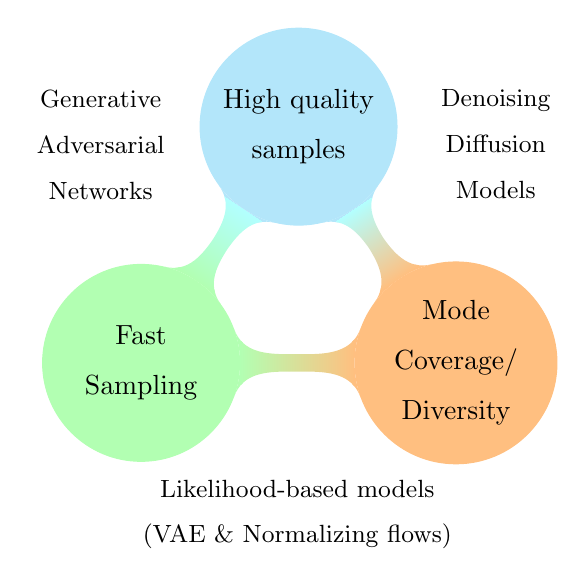
\begin{tikzpicture}[align=center]
		\node (entropy) at (0, 3) [concept, concept color=cyan!30, minimum size=2.5cm] {High quality \\samples};
		\node (enthalpy) at (2, 0) [concept, concept color=orange!50, minimum size=2.5cm] {Mode \\ Coverage/\\Diversity};
		\node (free-energy) at (-2, 0) [concept, concept color=green!30, minimum size=2.5cm] {Fast \\Sampling};
		
		\path (enthalpy) to[circle connection bar switch color=from (orange!50) to (green!30)] node[below=9ex, font=\small] {Likelihood-based models\\(VAE \& Normalizing flows)} (free-energy);
		\path (entropy) to[circle connection bar switch color=from (cyan!30) to (orange!50)] node[right=10ex, above=3ex, font=\small] {Denoising\\Diffusion\\Models} (enthalpy);
		\path (free-energy) to[circle connection bar switch color=from (green!30) to (cyan!30)] node[left=10ex, above=3ex, font=\small] {Generative\\Adversarial\\Networks} (entropy);
		
	\end{tikzpicture}
	\caption{Generative Learning Trilemma}
	\label{fig:related-generative-learning-trilemma}
	\end{figure}
	Since now, we have talked a lot about \gls{gan}s, but there are other architectures of generative models. We have seen that \gls{gan}s have serious problems with \textit{mode collapse}, which affects the diversity of synthetic data. While likelihood-based models and denoising diffusion models can cover a wide spectrum of possibilities, they suffer from low sample quality and thousands of network evaluations respectively. Most of the deep generative learning focus on high-quality definition, although all the requirements are highly important and key factors in a real environment. This is called the \textit{generative learning trilemma} \ref{fig:related-generative-learning-trilemma}.
	\\\\
	Likelihood-based models are alternatives to GANs that can cover a wide range of possibilities since they focus on estimating the likelihood or probability distribution of the data while training. There are several types of likelihood-based models although we will focus on \gls{vae}. The architecture of autoencoders are quite simple, they consist of an encoder, a smaller feature vector also called \textit{latent vector} $z$ and a decoder \ref{fig:related-autoencoder}. Therefore, the main goal of the encoder is to comprise the input vector $x$ while the decoder attempts to perform the conversion from lower to higher dimensional data, being the output vector $\bar{x}$. Hence, the best purpose of autoencoders is dimensionality reduction given its architecture. Then, the main purpose is to find the best set of encoder/decoder that keeps the maximum information with the less reconstruction error while decoding. In fact, one of the most popular usages of autoencoders in computer vision is the image reconstruction due to their architecture.
	\begin{figure}[H]
		\centering
		\includegraphics[width=10cm]{imgs/relatedwork/autoencoder}
		\caption{Autoencoder architecture.}
		\label{fig:related-autoencoder}
	\end{figure}
	\begin{figure}[H]
		\begin{align*}
			\mathcal{L}_{\text{MSE}} &= \frac{1}{N} \sum_{i=1}^{N} \| x_i - \bar{x}_i \|^2\\
				&= \frac{1}{N} \sum_{i=1}^{N} \| x_i - \text{decoder}(\text{encoder}(x_i)) \|^2
		\end{align*}
		\caption{MSE loss in autoencoders}
	\end{figure}
	Let's assume an autoencoder that both encoder and decoder have only one layer without non-linearity. In that sense, we can see clearly a link with PCA since we are looking for the best linear subspace to project data on with as few information loss as possible. However,  deep neural networks comes with also non-linear layers\footnote{Non-linear layers allow to learn complex relationships. Some of them are used as activation functions.}. The more complex of autoencoders architecture, the more they can proceed to a high dimensionality reduction while keeping the loss low. In an ideal case, if the encoder and the decoder have enough degrees of freedom and infinite power, the latent vector could be reduced to 1. Nevertheless, the dimensionality reduction comes with a price. First of all, we will lack of interpretable structures in the latent space. Secondly, the major part of the data structure information will not be in a reduced representation but in arbitrary one without any context of the patterns that the autoencoder could infer. Therefore, it is important to control and adjust the depth and the latent space dimensions depending on the final purpose.
	\\\\
	At this point, we have learned the surface from autoencoders, but how do they fit in image generation? Once the autoencoder has been trained, we have both encoder and decoder with the weights to reconstruct the data. At first, we might think that changing the latent vector we could take a point randomly from the space and decode it to get a new content. Although that could work, the regularity of the latent space for autoencoders is hard since it depends on several factors such as the data distribution, the latent space dimension and the architecture of the encoder. To sum up, there will be several biases that we are not able to control. 
	\\
	\\
	In order to make the latent vector regular and continuous, \gls{vae}s try to solve this problem by mapping the inputs to a normal probability distribution, so they introduce explicit regularization during the training process. Hence, the latent vector will be sampled from that distribution, being the decoder more robust at decoding latent vectors as a result. A \gls{vae} is an architecture composed of both encoder and decoder too. However, instead of encoding a latent vector, they encode it as a distribution over the latent space. The following enumeration details the process:
	\begin{enumerate}
		\item The input is encoded as a distribution over the latent space.
		\item A point is generated given the distribution encoded.
		\item The sampled point is decoded so the reconstruction and regularization error can be computed.
	\end{enumerate}
	The encoded distributions are chosen to be normal so that the encoder can be trained to return the mean and covariance matrix. This makes a way of both local and global regularization of the latent space respectively. Hence,the loss will not be only about the reconstruction of the data in the last layer, called \textit{reconstruction term}, but also how the latent space is organized by making the latent space close to a standard normal distribution, called the \textit{regularization term}. The latter will be calculated by how distant is from the gaussian distribution, using the \textit{Kullback-Leibler divergence}, which is expressed in terms of the means and the covariance matrices of the two distributions.
	\begin{figure}[H]
		\begin{align*}
			\mathcal{L}_{\text{VAE}} &= \text{Reconstruction term} &+&\qquad \text{Regularization term}\\
			&= (\frac{1}{N} \sum_{i=1}^{N} \| x_i - \bar{x}_i \|^2) &+& \qquad \sum_{j=1}^{J} \left(\mu_j^2 + \sigma_j^2  - \log(\sigma_j)  - 1 \right)
		\end{align*}
		\caption{Loss in \gls{vae}}
	\end{figure}
	To demonstrate the differences we can compare an autoencoder and a \gls{vae} trained by MNIST data, although it is a really balanced dataset. We can see in  that the range of values in the latent vector of the latter is much smaller and centralized, representing better any class. % TODO: REF!
	\subsubsection{Transformers in computer vision}
	\gls{cnn} have worked very well for cloud removal, but latest and disruptive state-of-the-art deep learning attention-based architectures \cite{VaswaniSPUJGKP17} uncover new paths to achieve remarkable improvements and results. It has been demonstrated that transformers can excellently overcome challenges such \gls{nlp} \cite{brown2020language}, Text-To-Image Generation \cite{pmlr-v139-ramesh21a}  or Image Completion \cite{pmlr-v119-chen20s} with large datasets, great model size and enough compute.
	\begin{figure}[H]
		\centering
		\includegraphics[width=7cm]{imgs/relatedwork/transformer-block}
		\caption{Transformer block architecture. \\
			\textbf{left block}, the encoder architecture, \textbf{right block}, the decoder architecture.}
		\label{fig:related-transformer-block}
	\end{figure}
	The transformer neural network is composed by an encoder-decoder architecture  much like \gls{rnn}. However, the difference is that the input sequence can be passed in parallel by passing also the positional encoder zipped with, as the input might have different meaning depending on its position. Therefore, the positional encoder is a vector that gives context based on position of the element in a sentence. \cite{VaswaniSPUJGKP17} uses the following sine and cosine function to generate this vector. For every odd step, they create the vector using the cosine function while for every even time step, they use the sine function. These functions have linear properties the model can easily learn to attend to when adding these vectors to their corresponding vector.
	\begin{align*}
	&PE(pos, 2i + 1) =cos(\frac{pos}{10000^{2i/dmodel}})\\
	&PE(pos, 2i) = sin(\frac{pos}{10000^{2i/dmodel}})
	\end{align*}
	The input and the positional encoding are passed into the encoder block. The job of the encoder is to map all input sequence into abstract continuous representation that holds the learned information for that entire sequence. The encoder block has $N$ identical encoder layers. Each layer has two sub-layers: a multi-head attention layer and a feed forward layer. Both sub-layers have a residual connection and a layer normalization\footnote{The normalization is done by each feature instead by each sample.} next to their output vector. The residual connections helps the network to train by allowing gradients to flow directly through the network while the normalization is used to stabilize the network.
	\begin{figure}[H]
		\centering
		\includegraphics[width=5cm]{imgs/relatedwork/transformer-multihead}
		\caption{Multi-Head Attention block}
		\label{fig:related-transformer-multi-head}
	\end{figure}
	Multi-head attention block applies a specific attention mechanism called self-attention, which allows the model to associate each individual element in the input to other elements. The attention is computed by how relevant is the \textit{i}\textsuperscript{th} element of the sentence to other words in the same sentence. This means that it is computing what part of the sentence should the model focus. Therefore, we can understand the attention as a vector that captures the contextual relationships between elements in the sentence.  To give the encoder model more representation power of the self-attention, the block is split into several blocks called heads, which can be run concurrently. The input of each head is fed into three distinct fully connected layers to create the query, key and value vectors. The idea is that the attention block must map the query against a set of keys to then present the best attention, which will be embedded to the values. In other words, the query is a vector related with what we encode, the key is a vector related with what we use as input to output and the value is the learned vector as a result of calculations but related with the input. Regarding encoder block, all three vectors are the source vector since what is wanted is to capture the attention of the elements between them.
	\begin{figure}[H]
		\centering
		\includegraphics[width=3.5cm]{imgs/relatedwork/transformer-scale-dot-product-attention}
		\caption{Scaled Dot Product Attention Head}
		\label{fig:related-transformer-head}
	\end{figure}
	To obtain self-attention, we will multiply the queries and the keys to obtain the score matrix, which determines how much focus should the $i^{th}$ element be put on the other elements so each element will have a score to correspond to other elements in the time step. The matrices will be scaled by $\sqrt{d_k}$, where $d_k$ is the dimension of the queries or the keys. This allows more stable gradients since multiplying values can have exploding effects. The softmax will turn the score matrix into a probabilistic matrix which any value is between 0 and 1 and the sum of each column or rows will be 1. A higher probability score means more focus. As it can be sensed, the scaled is also done because of the softmax and to prevent extremely small gradients. Finally, the attention score will be multiplied to the value vector and the result will be the output of the Scale Dot-Product Attention Head. Each output of the heads will be concatenated and then finally processed in a linear layer which output is the vector with encoded information on how each element should attend to all other elements in a sequence.
	\[Attention(Q, K, V) = softmax(\frac{QK^T}{\sqrt{d_k}}) V\]
	As it was said before, the other sub-layer of a encoder layer is the feed-forward layer, which is a network that is applied to the attention vectors. This layer is used to turn these vectors into a form that the next encoder or decoder block can get as an input so that it gives a richer representation to the next block.
	\\
	\\
	Regarding the decoder block, it has several similarities with the encoder block. They both have $N$ identical layers and a position encoding at first of all. However, multi-head attention layers of the decoder block have different job compared to the encoder. The decoder is auto-regressive and it takes the previous outputs from itself and the encoder output vector as inputs. This is because the encoder can use all the elements of the input sentence  but the decoder can only use the previous elements $\{ \, j\text{\textsuperscript{th} element} \, \, \, | \, \, \, j < i \, \}$ of the sentence. By not doing that, there would be no learning at all.
	Therefore, the first multi-head attention layer is masked so that it prevent it from being conditioned of the future tokens. In order to do that, once having the score matrix in a head, the result will be masked before calculating the softmax. Regarding the second multi-head attention layer, it can be seen that the queries and the keys are the encoder output while the values are the output of the first attention layer of the decoder, which also are the residual connection. Then, the result is passed into a feed forward layer for further processing and finally, goes to a linear layer that access a classifier and a softmax function to turn it into a probability distribution.
	\begin{table}[H]
		\centering
		\caption{Complexity per layer and number of sequential operations for different type layers. $n$ is the sequence length, $d$ is the representation dimension and $k$ is the kernel size of convolutions.}
		\begin{tabular}{c|cc}
			Layer Type & Complexity per layer & Sequential operations\\\hline
			Self-Attention & $O(n^2 \cdot d)$ & $O(1)$\\
			Recurrent & $O(n \cdot d^2)$ & $O(n)$ \\
			Convolutional &  $O(k \cdot n \cdot d^2)$ & O(1)\\
		\end{tabular}
	\end{table}
	Although transformers are great for sentence data such as text, its applications to computer vision problems do not fit as \gls{cnn} do, since the attention has a quadratic cost. For that reason, \cite{vit} created a self-attention architecture called \gls{vit} that can perform better in some cases than \gls{cnn}s reshaping the input to fit in the transformer architecture.
	\begin{figure}[H]
		\centering
		\includegraphics[width=12cm]{imgs/relatedwork/vit-architecture}
		\caption{\gls{vit} architecture}
	\end{figure}
	As it has been said, transformer's input is a 1D sequence. To turn the images into sequences, the 2D images $\{x | x \in \mathbb{R} ^{H \times W \times C}\}$ are reshaped into sequences of flattened 2D patches $\{x | x \in \mathbb{R}^{N \times (P^2 \times C)}\}$ to be handled, where $P$ is the resolution of each image patch and $N = \frac{HW}{P^2} $ is the number of patches. Therefore, $P$ is the input sequence length.
	Once the splitting is done, the patches are mapped to $D$ dimensions with a trainable linear projection, since the transformer encoder uses a constant latent vector of size $D$ through all of its layers. This process is called patch embedding. The positional embedding added to the patch embedding to retain positional information and to be fed to the transformer encoder.
	\\\\
	A more general way to understand \gls{vit} is that this architecture attempts to capture global attention of the image by putting the patches in the positional embedding while \gls{cnn} captures pixel attention over a kernel, understanding better by nature the textures of an image. Nowadays, \gls{vit}s are popular models to solve computer vision problems, since they can capture better global self-attention. However, if they are not trained on huge datasets, the best option is to stick to ResNet or EfficientNet, since in this case \gls{vit}s cannot outperform the \gls{cnn}s.
	Regarding image generation, in is proposed the ViTGAN with a Vanilla-\gls{vit} discriminator and a \gls{vit}-based generator, although a mixture of deconvolutional layers and global receptive fields form \gls{vit} might perform better.
	\\\\
	Regarding not only spatial but temporal computer vision challenges, \gls{ltae} is a network architecture that employs multi-headed self-attention mechanisms to classify remote sensing time sequences. In the \gls{tae}, the channels of the temporal inputs are distributed among several attention heads operating in parallel. Each head extracts highly-specialized temporal features which are in turn concatenated into a single representation. The proposed approach in \cite{garnot2021lightweight} modifies the \gls{tae} by distributing the channels of the temporal inputs among several compact attention heads operating in parallel, which allows for more efficient processing of time-series data.
	\begin{figure}[H]
		\centering
		\includegraphics[width=12cm]{imgs/relatedwork/ltae}
		\caption{\gls{ltae} architecture}
	\end{figure}
	The  \gls{tae} is a network architecture that employs multi-headed self-attention mechanisms to classify remote sensing time sequences. The channels of the temporal inputs are distributed among several attention heads operating in parallel. Each head extracts highly-specialized temporal features which are in turn concatenated into a single representation. The proposed approach modifies the \gls{tae} by distributing the channels of the temporal inputs among several compact attention heads operating in parallel, which allows for more efficient processing of time-series data. 
	\begin{figure}[H]
		\centering
		\includegraphics[width=15cm]{imgs/relatedwork/uncertainty}
		\caption{\cite{uncrtaints2021ebel} model generator architecture}
	\end{figure}
	This architecture is then used in \cite{uncrtaints2021ebel} to aggregate the information of temporal images without needing high computational resources. \cite{uncrtaints2021ebel} proposes a multi-temporal model using \cite{sen12mscrts} dataset, achieving the best results since now. Moreover, they add the paradigm of uncertainty in the field, being the first time to show how the well-calibrated predicted uncertainties
	enable a precise control of the reconstruction quality in the the task of multi-temporal
	cloud-removal in optical satellite images.

	% VQAE Difussion
	\subsection{Decision on thesis alignment}
	After reviewing the state-of-the-art proposals and the trend of current deep learning architectures, the objectives regarding model design process that align better in the context of this thesis due to the time and computation limitations are the following:
	\begin{itemize}
		\item Use \gls{sar} and Sentinel2 data in most of the model architectures since it is the most effective way to rmeove clouds.
		\item Train some models without \gls{sar} data and check the difference of it.
		\item Do not use architectures that need temporal data due to its training time, complexity and memory management.
		\item Try at least one of each type of generative models in the following order: \gls{vae}, \gls{gan} and denoising diffusion models.
		\item Try one \gls{gan} with a \gls{vit} as a discriminator and compare the behavior between other \gls{gan}.
	\end{itemize}
	\subsection{Academic Datasets}
	Several public datasets for cloud removal have been proposed over the recent years. In the following section, we will review a few of them and, finally, select those who are more aligned to the thesis and can be merged.
	\\
	\\
	The first public dataset published, called \texttt{RICE}, was described in \cite{rice}. Actually, it can be considered as two datasets, since there are two quite different parts: \texttt{RICE1} and \texttt{RICE2}. While \texttt{RICE1} contains 500 pairs of images\footnote{Each pair contains a cloudy and a cloudless image.} of $512 \times 512$ from Google Earth, \texttt{RICE2} contains 450 sets of images from Landsat 8 OLI/TIRS, being each set three images of $512 \times 512$ px: a cloudless image and a cloudy one with its mask. Compared to the following datasets, the size of both is relatively small and the data of them is spatio-temporal homogeneous. For that reason and since they are not from Sentinel-2, they have been discarded.
	\\
	\\
	\cite{sarukkai2019cloud} introduces two novel datasets contains nearly $10000$ paired Sentinel-2 images of $256 \times 256$ px	drawn from 17800 distinct tiles worldwide. The cloud cover for each cloudy image is between 10\% and 30\%. It excludes the images with insufficient visible ground upon manual inspection and they restrict the percentage of images of ocean being no more than 10 \% of the dataset. The other dataset contains 3130 sets of 3 cloudy images and a cloud-free image of the same region.
	\section{Exploratory Data Analysis}
	Once selected the datasets, an exploratory data analysis has been carried out to understand the hidden properties between bands from the images and the images themselves to gather enough information and make the dataset comprehensible so that the design and evaluation of deep learning models can be more straight-forward. Moreover, the EDA was aimed to provide insights into potential challenges that might be encountered during the development of the model. This stage of the thesis proposed four main challenges:
	\begin{itemize}
		\item Aggregating these datasets into a unified and standardized format is essential to ensure consistency and compatibility during the subsequent stages of the deep learning model development. Although they are meant to be aggregated at some point, a solution to fit the dataset schema into the actual challenge was needed.
		\item Extracting the properties using various techniques, including image processing algorithms and statistical analysis, without getting away from the main topic and attempting not to create biases while extracting the data.
		\item Visualizing the data can provide valuable insights but a huge amount of data extracted can be messy and create a high computational demand. 
		\item Understanding the limitations of the datasets, such as noise, class imbalance, or variations in image quality, allowed for the identification of potential biases and the formulation of suitable mitigation strategies.
	\end{itemize}
	During the EDA phase, various techniques were employed to extract meaningful information from the dataset. Descriptive statistics were computed to gain a preliminary understanding of the distribution, central tendency, and spread of the data across different bands. This provided an overview of the range and variability of values within each band, allowing for an initial assessment of their significance.
	By visually inspecting the images, patterns and trends specific to cloud formations must be discerned, aiding in the development of strategies to tackle cloud removal effectively. Furthermore, feature engineering techniques were explored to derive additional meaningful features from the dataset. This involved transforming, aggregating, or combining existing features to capture important characteristics of the data. After each information was discovered, this steps were not considered to be sequential but concurrent phases to incrementally learn and study the data. Therefore, the following subsections must be interpreted as chapters of a story of the analysis rather than separated and independent subsections.
	\subsection{Properties extraction and visualization of the first dataset}
	At first, I started creating a data exploration of \texttt{SEN12MS-CR} \cite{sen12mscr}), since it is the most aligned dataset. Once extracted and analyzed the data, merging it to the other data was thought to be more straight-forward.
	\\\\
	The first step to take at this stage was to take care of the pixel intensities in order to visualize and extract the information properly. The imagery values of each band were ranged from $0$ to $10000$. Therefore, the pixels need to be normalized and scaled for a proper processing and visualization of the data. This led to a challenge since I did not want to modify the images to the point that comparison or visualization of the properties extracted would be affected. Three normalization methods were thought:
	\begin{itemize}
		\item MinMax Scaling, also known as feature scaling, is a method that linearly transforms the pixel values of an image to a specific range, typically between 0 and 1. 
		\[\text{Normalized value} = \frac{\text{Pixel value} - \text{Min Value}}{\text{Max value} - \text{Min Value}}\]
		Although this preserves the distribution of the pixel intensities of images for processing, this method is not proper for visualization since outliers can affect the visualization of the data.
		\item Linear Stretch method. The linear stretch method is used to enhance the contrast of an image by stretching the pixel values across the a given available range.  If the pixel surpasses the 98\supindex{th} percentile, it will be 1 (or the maximum of the scaled vector). If the pixel value is under the 2\supindex{nd}, it will be 0 (or the minimum of the scaled vector). For the other pixel values, it performs the scaling operation by using interpolation, being the maximum value the 98\supindex{th} percentile and the 2\supindex{nd} the minimum.
		\[\text{Normalized value} = \frac{\text{Ranged pixel value} - \text{2\supindex{nd} percentile}}{\text{98\supindex{nd} percentile} - \text{2\supindex{nd} percentile}}\]
		\item Sigmoid after linear stretch method. The sigmoid after linear stretch method applies a sigmoid function to the linearly stretched pixel values to further enhance the contrast. In this formula, the slope $k$ is a parameter that controls the shape and position of the sigmoid function. The sigmoid function maps the stretched pixel values to a range between 0 and 1, enhancing the contrast in the process. By increasing the slope, the range of values can be compressed, so they get more blurred and with less contrast. This can be seen in  \ref{fig:eda-laplacian-vars-slope} and \ref{fig:eda-sigmoid-slope}.
		\[\text{Normalized value} = \frac{1}{1 + e^{-k \cdot(\text{LinearStretch}(\text{Pixel value}))}}\]
			\begin{figure}[H]
			\centering
			\includegraphics[width=9cm]{imgs/eda/sigmoid-slope-2}
			\caption{Laplacian variance depending on the slope used in sigmoid scaling method.}
			\label{fig:eda-laplacian-vars-slope}
		\end{figure}
	\end{itemize}
	The following pictures show how the images behave after treating each scaling method:
	\begin{figure}[H]
		\centering
		\includegraphics[width=15cm]{imgs/eda/scaled-methods-1}\\
		\includegraphics[width=15cm]{imgs/eda/scaled-methods-2}
		\caption{Scaling methods}
		\label{fig:scaling-methods}
	\end{figure}
	Regarding data processing for training, the best method to use is the MinMax feature scaling, since it preserves the intensity distribution and range of the values although its image visualization is poor.
	\\
	\\
	Regarding data visualization and general data extraction, although it seems in \ref{fig:scaling-methods} that the best normalization to apply is sigmoid after the linear stretch method, we can see in \ref{fig:eda-sigmoid-slope} that this would affect the study of the properties since the data would be so compressed that the analytical and visual results would not be as precise as it could. Therefore, the best method to carry out is the linear stretch method, since there are some pixel intensities that are outliers due to the noise or other obstacles while capturing the images.
	\\
	\\
	Moreover, it has been thought the normalization method as a parameter to use when training. The comparison of the methods will be useful to know which method is better to fit an image in a deep learning model.
	\begin{figure}[H]
		\centering
		\includegraphics[width=16cm]{imgs/eda/sigmoid-slope}
		\caption{Sigmoid-scaled images with their RGB bands in different slopes.}
		\label{fig:eda-sigmoid-slope}
	\end{figure}
	The properties compared in the first dataset are classified depending on how they were extracted:
	\begin{enumerate}
		\item Band properties of each image. Exploring properties related to individual bands helped to compare two bands given an image or different samples of images given these band properties.
		\begin{itemize}
			\item Descriptive statistics such as the mean, median, std and percentiles to compute  statistics for each band, providing insights into the distribution, central tendency, and spread of data values.
			\item Contrast. Analyzing the range and variation in pixel intensities within each band to understand the degree of contrast present. There are several ways to calculate contrast, the most popular ways are:
			\[\text{Traditional contrast} = \frac{\text{std}(\text{band})}{\text{mean}(\text{band})}\]
			\[\text{Michelson contrast} = \frac{\text{Maximum value} - \text{Minimum value}}{\text{Maximum value} + \text{Minimum value}}\]
			\item Blur. Assessing the level of blurriness in the images, indicating the sharpness of details captured. To extract the blurriness of the images, it has extracted the variance of the images after applying the laplacian filter.
			\item Kernel Density Estimation (KDE). KDE helped to visualize the probability density function of each band, aiding in the identification of underlying patterns or modes.
		\end{itemize}
		\item True Color Image (TCI) properties of each image. Although not all the bands captured from sentinel2 are visible in human spectra, comparing properties of the RGB bands could help us humans to understand the difference in the image captures.
		\begin{itemize}
			\item Saturation. Examining the saturation level of colors in the TCI, which indicates the vividness or intensity of hues. To get the saturation it has been changed from RGB to HSV color space.
			\item Temperature. Assessing the temperature or color balance of the TCI, providing information about the overall warmth or coolness of the image. To capture the temperature the images have been converted from RGB to CIE 1931 XYZ color space.
		\end{itemize}
		\item  The cloud coverage of each image was captured using the library  
		\begin{itemize}
			\item Percentage of each image. This quantifies the extent to which each image is covered by clouds, enabling the assessment of potential challenges posed by cloud interference.
			\item The MSE between cloud-free reference images and their corresponding cloudy versions was calculated allowing us for the evaluation of image quality degradation due to cloud cover.
		\end{itemize}
		\item An exploration of the indices showed in \ref{tab:sentinel2-bands} helped to reveal additional characteristics or features within the images and differences between the season and regions of interest.
	\end{enumerate}
	The analysis was ideal as a first step but hard to visualize due to the high amount of properties collected and its diversity of nature. Visualizations played a crucial role in revealing the inherent structure and characteristics of the dataset and for that reason, a first glance of the data should be done interactively. 
	Since the variability of the cases where to compare the dataset and how extremely hard was to visualize correctly and effectively all the properties data extracted, the best decision to make was creating a web app to help the user experience of the EDA. 
	\\
	\\
	The app is powered by Streamlit. The library is a powerful and user-friendly python library that simplifies the process of building interactive web applications for data analysis and machine learning. It provides a straightforward way to create custom web interfaces directly from Python scripts, enabling users to easily visualize and explore data, create interactive dashboards, and share their work with others.
	\\\\
	Streamlit works by allowing developers to write Python code that defines the various components of the web application, such as widgets, plots, and text. These components are then rendered in a web browser, creating an intuitive and interactive user interface. The library takes care of handling the communication between the Python backend and the frontend, making it seamless for users to interact with the application.
	\\\\
	
	\subsection{Analysis}
	\subsection{Conclusions}
	
	\section{Model training pipeline}
	% MLFLOw
	% DataParallel
	% ModelParallel
	\section{Experiments \& results}
	\section{Conclusions}
	\section{Bibliography}

	\bibliography{bibliography}
	\bibliographystyle{unsrt}\end{document}